\section{Flux pulse shape correction}

\begin{figure}[htbp]
    \centering
    \makebox[\textwidth][c]{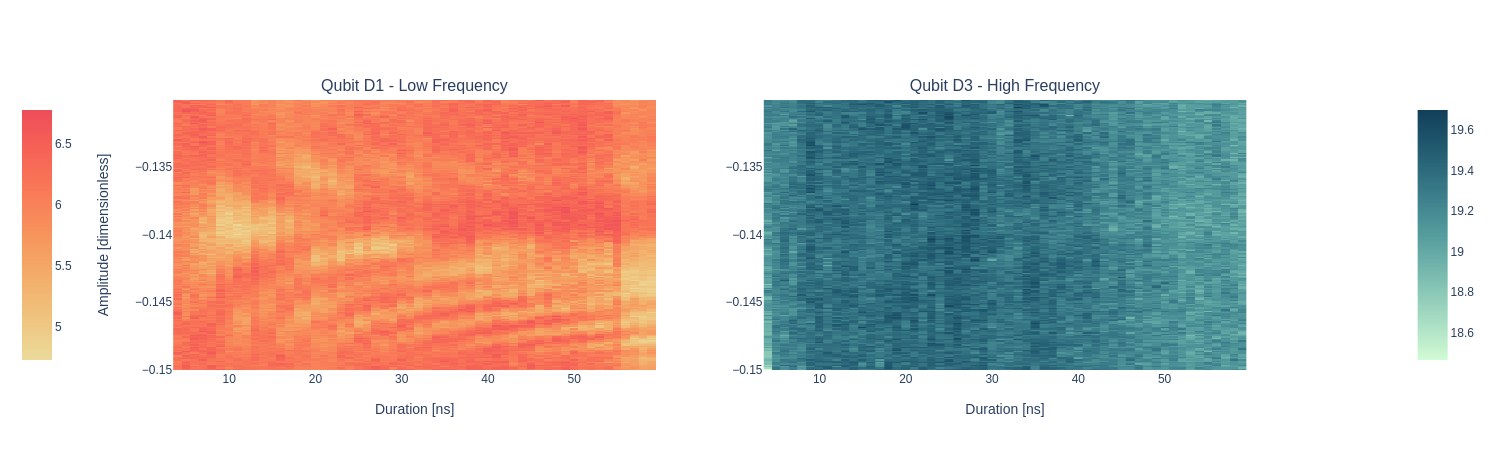
\includegraphics[width=1.3\textwidth]{Two-qubits calibration/Figures/chevron_bad.png}}
    \caption{Chevron plot for CZ. The distortion, that will be fixed in the next section, causes the asymmetry higher-lower bias. The leakage causes the chevron to not close and to not appear in the high frequency qubit.}
    \label{fig:chevron_distorted}
\end{figure}

The result of the last experiment should be exactly symmetric, as presented in \cref{fig:chevron_sketch}, but this is hardly the case.
Usually the result is much more distorted as presented in \cref{fig:chevron_distorted}, for example.

The problem in this case is the effective shape of the flux pulse.
We are now sending a rectangular pulse, with the idea that we can use it to perform a jump between two different flux values, without any transients.
In reality, the pulse gets partially deformed by the quality of the line, in particular its capacitance, that transform the pulse from a rectangular to something like what is presented in \cref{fig:rectangular_distortion}.

\begin{figure}[ht]
    \centering
    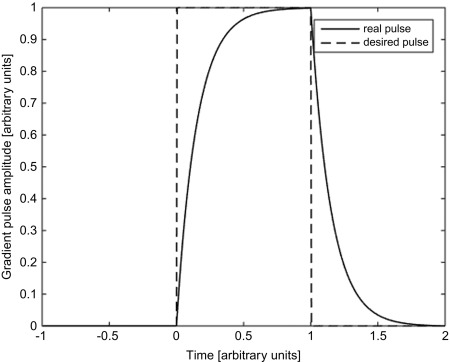
\includegraphics[width=6cm]{Two-qubits calibration/Figures/rectangular_distortion.jpg}
    \caption{Rectangular pulse distortion.}
    \label{fig:rectangular_distortion}
\end{figure}

The solution to this problem is to change the shape of the flux pulse to an ideal rectangular to something that will produce an effective rectangular~\cite{Rol2020, Ferreira2022}.
To achieve this, there are different possibilities, but the most straightforward consists in just implementing a new pulse shape and fine tune it manually using the symmetry of the chevron plot of the last experiment as figure of merit.

A sensible ansatz for the flux pulse is presented in \cref{eq:exponential-flux}.
\begin{equation}\label{eq:exponential-flux}
    y = A * \frac{(\exp(-x/\upsilon)) + g * \exp(-x/\tau)}{1+g}
\end{equation}
where basically the rectangular pulse is corrected with an initial exponential function, to counter the initial transient.



